
\documentclass{article}
\usepackage[spanish]{babel} %Definir idioma español
\usepackage[utf8]{inputenc} %Codificacion utf-8
\usepackage{amssymb, amsmath, amsbsy, wasysym}
\usepackage{multirow} % para tablas
\usepackage{graphicx}
\usepackage[ruled, vlined, spanish, linesnumbered]{algorithm2e} %Para escribir algoritmos
\title{Tarea 4\\Algoritmos}
\author{Emmanuel Peto Gutiérrez\\José Luis Vázquez Lázaro}
\begin{document}
\maketitle

\section*{Problema 4}

\textbf{a)}

Se recibe una gráfica $G=(V,E)$ y se construye una gráfica $G' = (V,E')$, donde el conjunto de aristas $E'$ es el mismo que $E$ pero sus aristas tienen como peso el inverso aditivo de su correspondiente en $E$. Es decir, si $uv$ es una arista de $E$ con peso $p$, entonces $uv$ está en $E'$ pero su peso es $-p$.

Se ejecuta el algoritmo de Kruskal sobre $G'$ para obtener un árbol generador de peso mínimo $T'$. Luego, se construye un árbol $T$ con las mismas aristas de $T'$ pero con el inverso aditivo de los pesos. Así, el árbol $T$ es el árbol generador de peso máximo de $G$.

\begin{algorithm}[htbp]
\SetKwInput{Entrada}{Entrada}
\Entrada{Una gráfica $G$ en su representación de lista de aristas.}
\SetKwInput{Salida}{Salida}
\Salida{Lista de aristas $T$ que forman un árbol generador de peso máximo de $G$.}

$E' = \emptyset$\;
\For{$(uv,p) \in E$}{
    $E'$.\textsc{Add}($(uv,-p)$)\;
}
$G' = (V, E')$\;
$T' =$ \textsc{Kruskal}($G'$)\;
$T = \emptyset$\;
\For{$(uv,p) \in T'$}{
    $T$.\textsc{Add}($(uv,-p)$)\;
}

\caption{\textsc{ArbolMaximo($G=(V,E)$)}}

\end{algorithm}

\textbf{b)}

Gráfica $G'$:

\begin{center}
\includegraphics[scale=1]{kruskal/p1}
\end{center}

Ejecución:

\begin{center}
1)\includegraphics[scale=1]{kruskal/p2}
\hspace{10mm}
2)\includegraphics[scale=1]{kruskal/p3}
\end{center}

\begin{center}
3)\includegraphics[scale=1]{kruskal/p4}
\hspace{10mm}
4)\includegraphics[scale=1]{kruskal/p5}
\end{center}

\begin{center}
5)\includegraphics[scale=1]{kruskal/p6}
\hspace{10mm}
6)\includegraphics[scale=1]{kruskal/p7}
\end{center}

\begin{center}
7)\includegraphics[scale=1]{kruskal/p8}
\hspace{10mm}
8)\includegraphics[scale=1]{kruskal/p9}
\end{center}

De los pasos 1) al 7) es la ejecución del algoritmo de Kruskal. Del paso 7) al 8) es la construcción del árbol de peso máximo $T$ a partir de $T'$.

\textbf{c)}

Se tiene como precondición que $G$ tiene solamente pesos no negativos, así que la gráfica $G'$ solo tendrá aristas con pesos menores o iguales a 0. Al ejecutar el algoritmo de Kruskal se agregan las aristas en orden creciente (siempre que no se forme un ciclo), y dado que todas serán negativas se toman primero las aristas cuyo valor absoluto es el mayor.

Al terminar el algoritmo, se tendrá un árbol $T'$ y $w(T') = p$. Por la correctitud del algoritmo de Kruskal se tiene que cualquier otro árbol generador de $G'$ tendrá un peso mayor o igual a $p$. Como todas las aristas de $G'$ son negativas, cualquier árbol generador $U$ de $G'$ tendrá peso negativo y como $w(T')$ es el menor de esos pesos, entonces $|w(T')| \geq |w(U)|$.

Por la construcción de $T$, se tiene que $w(T) = |w(T')|$. $T$ es un árbol generador de $G$ y para cualquier otro árbol generador $S$ de $G$ se tendrá que $w(S) \leq w(T)$, y por lo tanto $T$ es un árbol generador de peso máximo de $G$. $\blacksquare$

\textbf{d)}

Se va a suponer que la gráfica está en su representación por lista de aristas y que el algoritmo de Kruskal usa la estructura de datos Union-Find optimizada. El orden de la gráfica es $n$ y su tamaño es $m$.

\begin{itemize}
\item Construir la gráfica $G'$ a partir de $G$ toma tiempo $\Theta(m)$.
\item Ejecutar el algoritmo de Kruskal toma tiempo $O(m \log n)$.
\item Construir $T$ a partir de $T'$ toma tiempo $\Theta(n)$, pues un árbol generador tiene $n-1$ aristas.
\end{itemize}

Entonces la complejidad es $O(m \log n + m + n)$. Como el término que crece más rápido es $m \log n$ se puede decir que la complejidad es $O(m \log n)$.

\section*{Problema 5}

\textbf{a)}

Se va a suponer que la entrada es una gráfica $G$ con pesos en su representación con listas de adyacencias. Cada elemento en una lista de adyacencias de $v$ es un par $(u,p)$, donde $u$ es un vecino de $v$ y $p$ es el peso de la arista $vu$. También se supone que existe una función \textsc{EsConexa} que recibe una gráfica en su representación por listas de adyacencias y devuelve 1 si es conexa y 0 si no lo es.

El algoritmo se ejecuta de la siguiente forma.

\begin{itemize}
\item[1)] Recorrer las listas de adyacencias de todos los vértices. Si se encuentra un par $(u,p)$ tal que $p > b$, entonces se elimina al elemento $(u,p)$ de la lista.
\item[2)] Al terminar el paso 1) se tendrá una subgráfica generadora $H \subseteq G$. Ejecutar la función \textsc{EsConexa} sobre $H$ y devolver el mismo valor de retorno de la función \textsc{EsConexa}.
\end{itemize}

\textbf{Nota:} La función \textsc{EsConexa} se puede crear de la siguiente manera: inicialmente se marcan todos los vértices como \textit{no visitado} (puede ser un atributo booleano del vértice). Ejecutar DFS sobre la gráfica, a partir de un vértice arbitrario, y marcar como \textit{visitado} los que se visiten por el algoritmo DFS. Si todos los vértices están marcados como visitados entonces se devuelve 1, en otro caso se devuelve 0.

En el Algoritmo \textsc{CuelloDeBotella} se muestra un pseudocódigo que resuelve el problema. Cada vértice $v$ tiene una lista de sus vecinos llamada $ady$. Se utiliza un iterador para recorrer las listas de adyacencias, la función \textsc{Next()} devuelve al siguiente elemento en la lista y la función \textsc{Delete()} elimina al último elemento devuelto.\footnote{Este iterador funciona como el \textit{ListIterator} de Java.}

\begin{algorithm}[htbp]
\SetKwInput{Entrada}{Entrada}
\Entrada{Una gráfica $G$ en su representación por listas de adyacencias y un número $b$.}
\SetKwInput{Salida}{Salida}
\Salida{1 si existe una subgráfica generadora conexa donde cada arista tiene peso a lo más $b$; 0 en otro caso.}
\For{$v \in V$}{
    iterador = $v.ady$.\textsc{ListIterator()}\;
    \While{$iterador.$\textsc{HasNext}$()$}{
        par = iterador.\textsc{Next}()\;
        \If{$par.peso > b$}{
            iterador.\textsc{Delete}()\;
        }
    }
}
return \textsc{EsConexa}($G$)\;
\caption{\textsc{CuelloDeBotella($G=(V,E), b$)}}

\end{algorithm}

\textbf{b)}

En una gráfica no dirigida, en la representación de listas de adyacencias, para cada arista $uv \in E$, $u$ aparece en la lista de adyacencias de $v$ y $v$ aparece en la lista de adyacencias de $u$. Sin embargo, para reducir el número de figuras en esta tarea se hará una simplificación: cada vez que se borre al vértice $v$ de la lista de $u$, también se va a borrar $u$ de la lista de $v$, entendiendo que en el algoritmo real la segunda eliminación puede ocurrir varias iteraciones después. Tampoco se mostrará la ejecución del algoritmo DFS (de la función \textsc{EsConexa}).

En el algoritmo se revisan todas las aristas, y para seguir la pista del algoritmo se va a sombrear de gris la arista que se está revisando en la iteración actual.

\begin{center}
1)\includegraphics[scale=0.6]{bottleneck/g1}
\hspace{5mm}
\includegraphics[scale=0.9]{bottleneck/l1}
\end{center}

\begin{center}
2)\includegraphics[scale=0.6]{bottleneck/g2}
\hspace{5mm}
\includegraphics[scale=0.9]{bottleneck/l2}
\end{center}

\begin{center}
3)\includegraphics[scale=0.6]{bottleneck/g3}
\hspace{5mm}
\includegraphics[scale=0.9]{bottleneck/l3}
\end{center}

\begin{center}
4)\includegraphics[scale=0.6]{bottleneck/g4}
\hspace{5mm}
\includegraphics[scale=0.9]{bottleneck/l4}
\end{center}

\begin{center}
5)\includegraphics[scale=0.6]{bottleneck/g5}
\hspace{5mm}
\includegraphics[scale=0.9]{bottleneck/l5}
\end{center}

\begin{center}
6)\includegraphics[scale=0.6]{bottleneck/g6}
\hspace{5mm}
\includegraphics[scale=0.9]{bottleneck/l6}
\end{center}

\begin{center}
7)\includegraphics[scale=0.6]{bottleneck/g7}
\hspace{5mm}
\includegraphics[scale=0.9]{bottleneck/l7}
\end{center}

\begin{center}
8)\includegraphics[scale=0.6]{bottleneck/g8}
\hspace{5mm}
\includegraphics[scale=0.9]{bottleneck/l8}
\end{center}

\begin{center}
9)\includegraphics[scale=0.6]{bottleneck/g9}
\hspace{5mm}
\includegraphics[scale=0.9]{bottleneck/l9}
\end{center}

\begin{center}
10)\includegraphics[scale=0.6]{bottleneck/g10}
\hspace{5mm}
\includegraphics[scale=0.9]{bottleneck/l10}
\end{center}

\begin{center}
11)\includegraphics[scale=0.6]{bottleneck/g11}
\hspace{5mm}
\includegraphics[scale=0.9]{bottleneck/l11}
\end{center}

\begin{center}
12)\includegraphics[scale=0.6]{bottleneck/g12}
\hspace{5mm}
\includegraphics[scale=0.9]{bottleneck/l12}
\end{center}

\begin{center}
13)\includegraphics[scale=0.6]{bottleneck/g13}
\hspace{5mm}
\includegraphics[scale=0.9]{bottleneck/l13}
\end{center}

\begin{center}
14)\includegraphics[scale=0.6]{bottleneck/g14}
\hspace{5mm}
\includegraphics[scale=0.9]{bottleneck/l14}
\end{center}

\begin{center}
15)\includegraphics[scale=0.6]{bottleneck/g15}
\hspace{5mm}
\includegraphics[scale=0.9]{bottleneck/l15}
\end{center}

\begin{center}
16)\includegraphics[scale=0.6]{bottleneck/g16}
\hspace{5mm}
\includegraphics[scale=0.9]{bottleneck/l16}
\end{center}

\begin{center}
17)\includegraphics[scale=0.6]{bottleneck/g17}
\hspace{5mm}
\includegraphics[scale=0.9]{bottleneck/l17}
\end{center}

\begin{center}
18)\includegraphics[scale=0.6]{bottleneck/g18}
\hspace{5mm}
\includegraphics[scale=0.9]{bottleneck/l18}
\end{center}

\begin{center}
19)\includegraphics[scale=0.6]{bottleneck/g19}
\hspace{5mm}
\includegraphics[scale=0.9]{bottleneck/l19}
\end{center}

\begin{center}
20)\includegraphics[scale=0.6]{bottleneck/g20}
\hspace{5mm}
\includegraphics[scale=0.9]{bottleneck/l20}
\end{center}

\begin{center}
21)\includegraphics[scale=0.6]{bottleneck/g21}
\hspace{5mm}
\includegraphics[scale=0.9]{bottleneck/l21}
\end{center}

\begin{center}
22)\includegraphics[scale=0.6]{bottleneck/g22}
\hspace{5mm}
\includegraphics[scale=0.9]{bottleneck/l22}
\end{center}

\begin{center}
23)\includegraphics[scale=0.6]{bottleneck/g23}
\hspace{5mm}
\includegraphics[scale=0.9]{bottleneck/l23}
\end{center}

En este caso, la subgráfica resultante no es conexa, así que se devuelve 0.

\textbf{c)}

El problema consiste en decidir si existe una subgráfica generadora $H$ de $G$, conexa, tal que todas las aristas de $H$ tienen peso menor o igual a $b$. Dicho de otra forma, una subgráfica generadora $H$ de $G$ que cumpla esas propiedades no puede tener ninguna arista cuyo peso sea mayor que $b$.

Lo que hace el algoritmo es borrar de $G$ todas las aristas de peso mayor a $b$ y después comprobar si la gráfica resultante es conexa. Digamos que $G'$ es el resultado de elmininar todas esas aristas. Si $G'$ es conexa entonces se devuelve 1, pues $G'$ cumple con las propiedades de: generar a $G$, ser conexa y tener solo aristas de peso menor o igual a $b$. De hecho, cualquier subgráfica generadora y conexa de $G'$ cumple con esa propiedad.

Si $G'$ no es conexa el algoritmo devuelve 0. Nótese que $G'$ es una subgráfica generadora maximal con la propiedad de tener aristas de peso a lo más $b$. Así que cualquier subgráfica generadora de $G$ que sólo tenga aristas de peso a lo más $b$ será subgráfica de $G'$, y como $G'$ no es conexa, entonces cualquier subgráfica generadora de $G'$ tampoco lo será. Por lo tanto, no puede existir una subgráfica generadora de $G$, conexa, que tenga solo aristas de peso menor o igual a $b$, y por lo tanto el algoritmo devuelve el resultado correcto. $\blacksquare$

\textbf{d)}

\begin{itemize}
\item Recorrer todas las listas de adyacencias tiene complejidad $O(n+m)$.
\item Si se utilizan listas ligadas, la operación de eliminar (\textsc{Delete()}) del iterador toma tiempo $O(1)$. En el peor caso se realizarán $O(n+m)$ eliminaciones.
\item La función \textsc{EsConexa} toma tiempo $O(n+m)$, pues ejecutar DFS en una gráfica en su representación por listas de adyacencias toma tiempo $O(n+m)$ y ver si todos los vértices fueron visitados toma tiempo $O(n)$.
\end{itemize}

Así, el algoritmo toma tiempo total $O(n+m)$.

\end{document}

